\documentclass[12pt, a4paper, onecolumn, oneside, toc=bibliographynumbered, liststotoc]{scrreprt} %Schriftgröße 12pt, DIN A4, 1 Spalte, einseitig bedruckt, Literaturverzeichnis in Inhaltsverzeichnis eintragen mit Nummerierung als Anhang

\usepackage[T1]{fontenc} %Codierung für deutsche Schriftzeichen
\usepackage[utf8]{inputenc} % UTF-8 Encoding
\usepackage[ngerman]{babel} % Neue Deutsche Rechtschreibung
\usepackage[onehalfspacing]{setspace} %1,5 Zeilen Zeilenabstand
\usepackage{scrlayer-scrpage} %Kontrolle von Fuß- und Kopfzeile
\usepackage{graphicx} %Einfügen von Bildern
\usepackage{float} %Positionierung von Bildern
\usepackage[printonlyused, nohyperlinks, smaller]{acronym} %Unterstützung für Abkürzungen und Abkürzungsverzeichnis - es werden nur verwendete Abk. gedruckt
\pagestyle{scrheadings} %Seitenstil
\chead*{\pagemark} %Kopfzeile Mitte - Seitenzahl
\cfoot*{} %Fußzeile Mitte - leer
\usepackage{geometry}
\geometry{
  left=4cm,
  right=2cm,
  top=2cm,
  bottom=2cm,
%  bindingoffset=5mm
}
\usepackage[german=quotes]{csquotes}
\usepackage[backend=bibtex, citestyle=authoryear, bibstyle=authoryear, sorting=nty]{biblatex} %Angaben für Zitate - Nutzt Bibtex, Markierung auf Seite als alphanumerische Abkürzung, Sortierung nach Auftreten
\setcounter{biburllcpenalty}{9000}
\setcounter{biburlucpenalty}{9000}
\counterwithout{figure}{chapter}
\counterwithout{table}{chapter}
\addbibresource{Aufgabe_1.bib} %Bibliotheksdatei
%\addbibresource{WissArb.bib} %Bibliotheksdatei
% !!! Um Bibtex richtig zu verwenden, nach jeder Änderung in der .bib-Datei Bibtex laufen lassen !!!

%\setcounter{tocdepth} {4} % Inhaltsverzeichnis bis subsubsection
%\setcounter{secnumdepth}{4} % Nummerierung des Inhaltsverzeichnis bis subsubsection

\begin{document}
%Titelblatt und Inhaltsverzeichnis
\pagenumbering{roman} %Seitennummerierung i, ii, iii etc. 
	%Angaben für Maketitle
	\titlehead{Hochschule Rhein-Waal \\ %Hochschulinformationen
	Fakultät: Kommunikation und Umwelt\\
	Studiengang: Verwaltungsinformatik\\
	Modul: Workshop 2: Wissenschaftliches Schreiben\\}
%	\subject{Wissenschaftliches Arbeiten} %Art der Arbeit
	\title{Aufgabe 4\\
	Hausarbeit} %Titel
%	\subtitle{Einfallstore für Black Hat Hacker in Netzwerke} %Untertitel
	\author{Linus Wolf - 28611}
	\date{\today} %Datum (heute)
%	\publishers{Betreut durch Professor Frank Zimmer} %Betreuender Professor und zusätzliche Infos

\maketitle %Erzeuge Titelblatt (Ignoriert in scrreprt voreingestellte Kopf- und Fußzeile)
\newpage

%\newpage %Ende Abstract
\tableofcontents %Erzeuge Inhaltsverzeichnis (Bei Fehler erneut kompilieren - ToC braucht 2 Durchläufe)
\newpage

\listoffigures %Abbildungsverzeichnis
\newpage %Abschluss Titel und ToC - Neue Seite für Inhalt

\pagenumbering{arabic} %Seitennummerierung 1, 2, 3 etc. - Startet neu bei 1

	\chapter{Einleitung}
Laut Statista haben 2021 bereits 10,49 Millionen Haushalte mindestens ein Smart Home Gerät und es werden immer mehr. Für 2025 werden 18,45 Millionen Haushalte prognostiziert.

\begin{figure}[H]
	\centering
	\caption{Prognose zur Anzahl von Smart Home Haushalten in Deutschland} % \\ \parencite{Statista.2021}}
	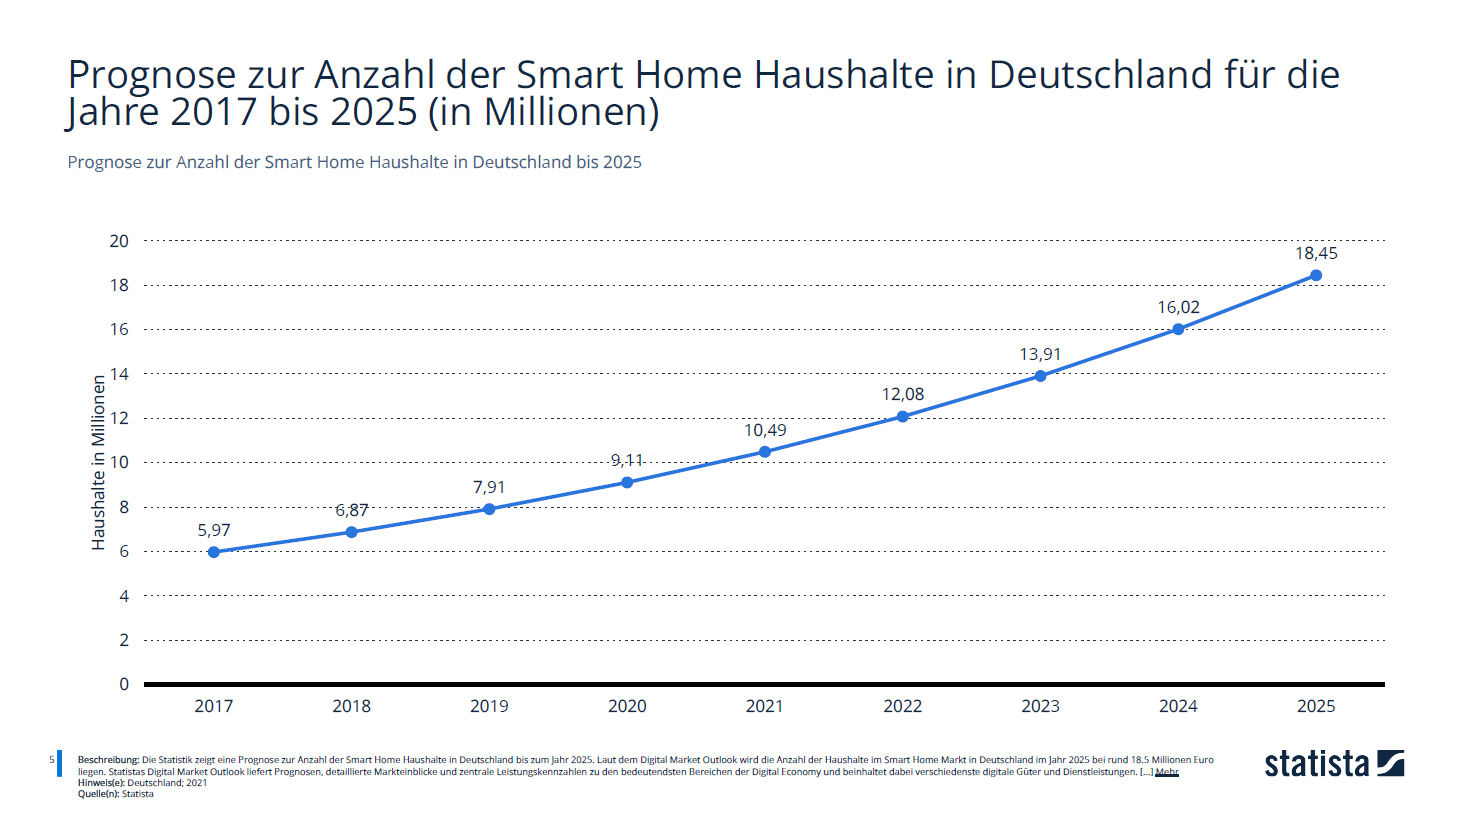
\includegraphics[width=0.9\textwidth]{AnzahlSmartHomeHaushalteStatista}
	\label{AnzahlGeräte}
\end{figure}

Die vielfältige Auswahl an Geräten lässt bereits heute nur noch wenige Wünsche offen. Kühlschränke, Kaffeemaschinen, Leuchtmittel, Sicherheitstechnik, Überwachungstechnik, Gartengeräte, Saugroboter, Lautsprecher und Sprachassistenten wie Alexa, Siri und Cortana. Aber auch persönliche medizinische Geräte wie Insulinpumpen oder implantierte Blutzuckermessgeräte oder Herzschrittmacher sind verbreitet. Fast alle verwenden WLAN, Bluetooth oder ein anderes Funkprotokoll, um mit Basisstationen oder Apps zu kommunizieren.

Dadurch sind sie Teil des Internet of Things (IoT) und damit auch von außerhalb des eigenen Netzwerks auffindbar und angreifbar. Im Jahr 2018 warnte das Bundesamt für Sicherheit in der Informationstechnik (BSI) im seinem jährlich erscheinenden Bericht zur Lage der IT-Sicherheit in Deutschland das IoT-Geräten \textquote[{\cite[21]{BundesamtfurSicherheitinderInformationstechnik.20210106b}}]{in der Regel
deutlich knappere Ressourcen für Sicherheitsmechanismen zur Verfügung stehen. IoT-Geräte können darum nicht nur einfacher kompromittiert werden, es ist auch deutlich schwerer, diese Kompromittierungen zu erkennen}.

In diesem Paper soll ein Überblick gegeben werden über mögliche Angriffsmethoden auf Smart Home Geräte und den Nutzen, der aus diesen Angriffen gezogen werden kann.

	\chapter{Dauerhafte Erreichbarkeit von Smart Home Geräten}
        Immer mehr Menschen benutzen Geräte und Dienste zur Steuerung und Überwachung ihres Zuhauses. Dauerhafte Erreichbarkeit bedeutet, dass ein Smart Home Gerät jederzeit über das Internet erreichbar ist und Befehle von einem Smartphone oder einem anderen Gerät aus empfangen kann. Es gibt jedoch einige Herausforderungen bei der dauerhaften Erreichbarkeit von Smart Home Geräten. Zum Beispiel kann die Internetverbindung manchmal unzuverlässig sein oder es können Probleme mit den Geräten selbst auftreten. Es ist wichtig, dass Hersteller von Smart Home Geräten Maßnahmen ergreifen, um die Dauerhafte Erreichbarkeit ihrer Geräte zu verbessern und Probleme zu beheben, wenn sie auftreten.
        
        Smart Home Geräte kommunizieren über eine Vielzahl von Technologien und Protokollen, abhängig von ihren Funktionen und ihrem Einsatzbereich. Einige Smart Home Geräte können auch über mehrere Technologien und Protokolle kommunizieren, um die Kompatibilität mit verschiedenen Geräten und Systemen zu verbessern. 
    
		\section{Mash-Netzwerk}
            Der IEEE 802.11-Standard, welcher für \enquote{Standard für Informationstechnologie - Telekommunikation und Informationsaustausch zwischen Systemen - Lokale und Metropolen-Netzwerke - Spezifische Anforderungen Teil 11: Wireless LAN Medium Access Control (MAC) und Physical Layer (PHY) Spezifikationen} steht, hat für die Verwendung von Mesh-Netzwerken eine eigene Bezeichnung: IEEE 802.11s. Hierbei kommt es zu den oben genannten Titel der Zusatz \enquote{Änderung 10: Mesh-Netzwerk}. Beim IEEE 802.11s wird ein neues Routing-Verfahren eingesetzt, welches auf der MAC-Schicht anstatt auf der Netzwerkschicht, wie beim \enquote*{traditionellen} IEEE 802.11, durchgeführt wird. Dabei behält der IEEE 802.11s-Standard die physischen Schichten wie bei dem „traditionellen“ Standard. Um ein effizientes Routing zu haben, müssen die Knoten genaue Kenntnisse über die drahtlosen Verbindungen haben, die sie mit ihren direkten Nachbarn verbinden. Dies führt zu nahtlosem Routing für Protokolle höherer Schichten. In einem IEEE 802.11s-Mesh-Netzwerk, auch als Mesh Basic Service Set (MBSS) bezeichnet, gibt es verschiedene logische Komponenten, wie in Abbildung 1 dargestellt. Die wichtigsten sind die Mesh-Stationen (Mesh STAs), die an der Bildung des MBSS teilnehmen und in dem jeder Knoten die gleiche Komplexität hat und keine hierarchische Struktur vorliegt. Die Mesh STAs nehmen außerdem an der Pfadauswahl und -weiterleitung teil, wodurch ein sehr einfaches selbstorganisiertes Netzwerk entsteht.

            \begin{figure}[htpb]
           	\centering
	           \caption{Architektur eines Mesh-Netzwerkes}
	           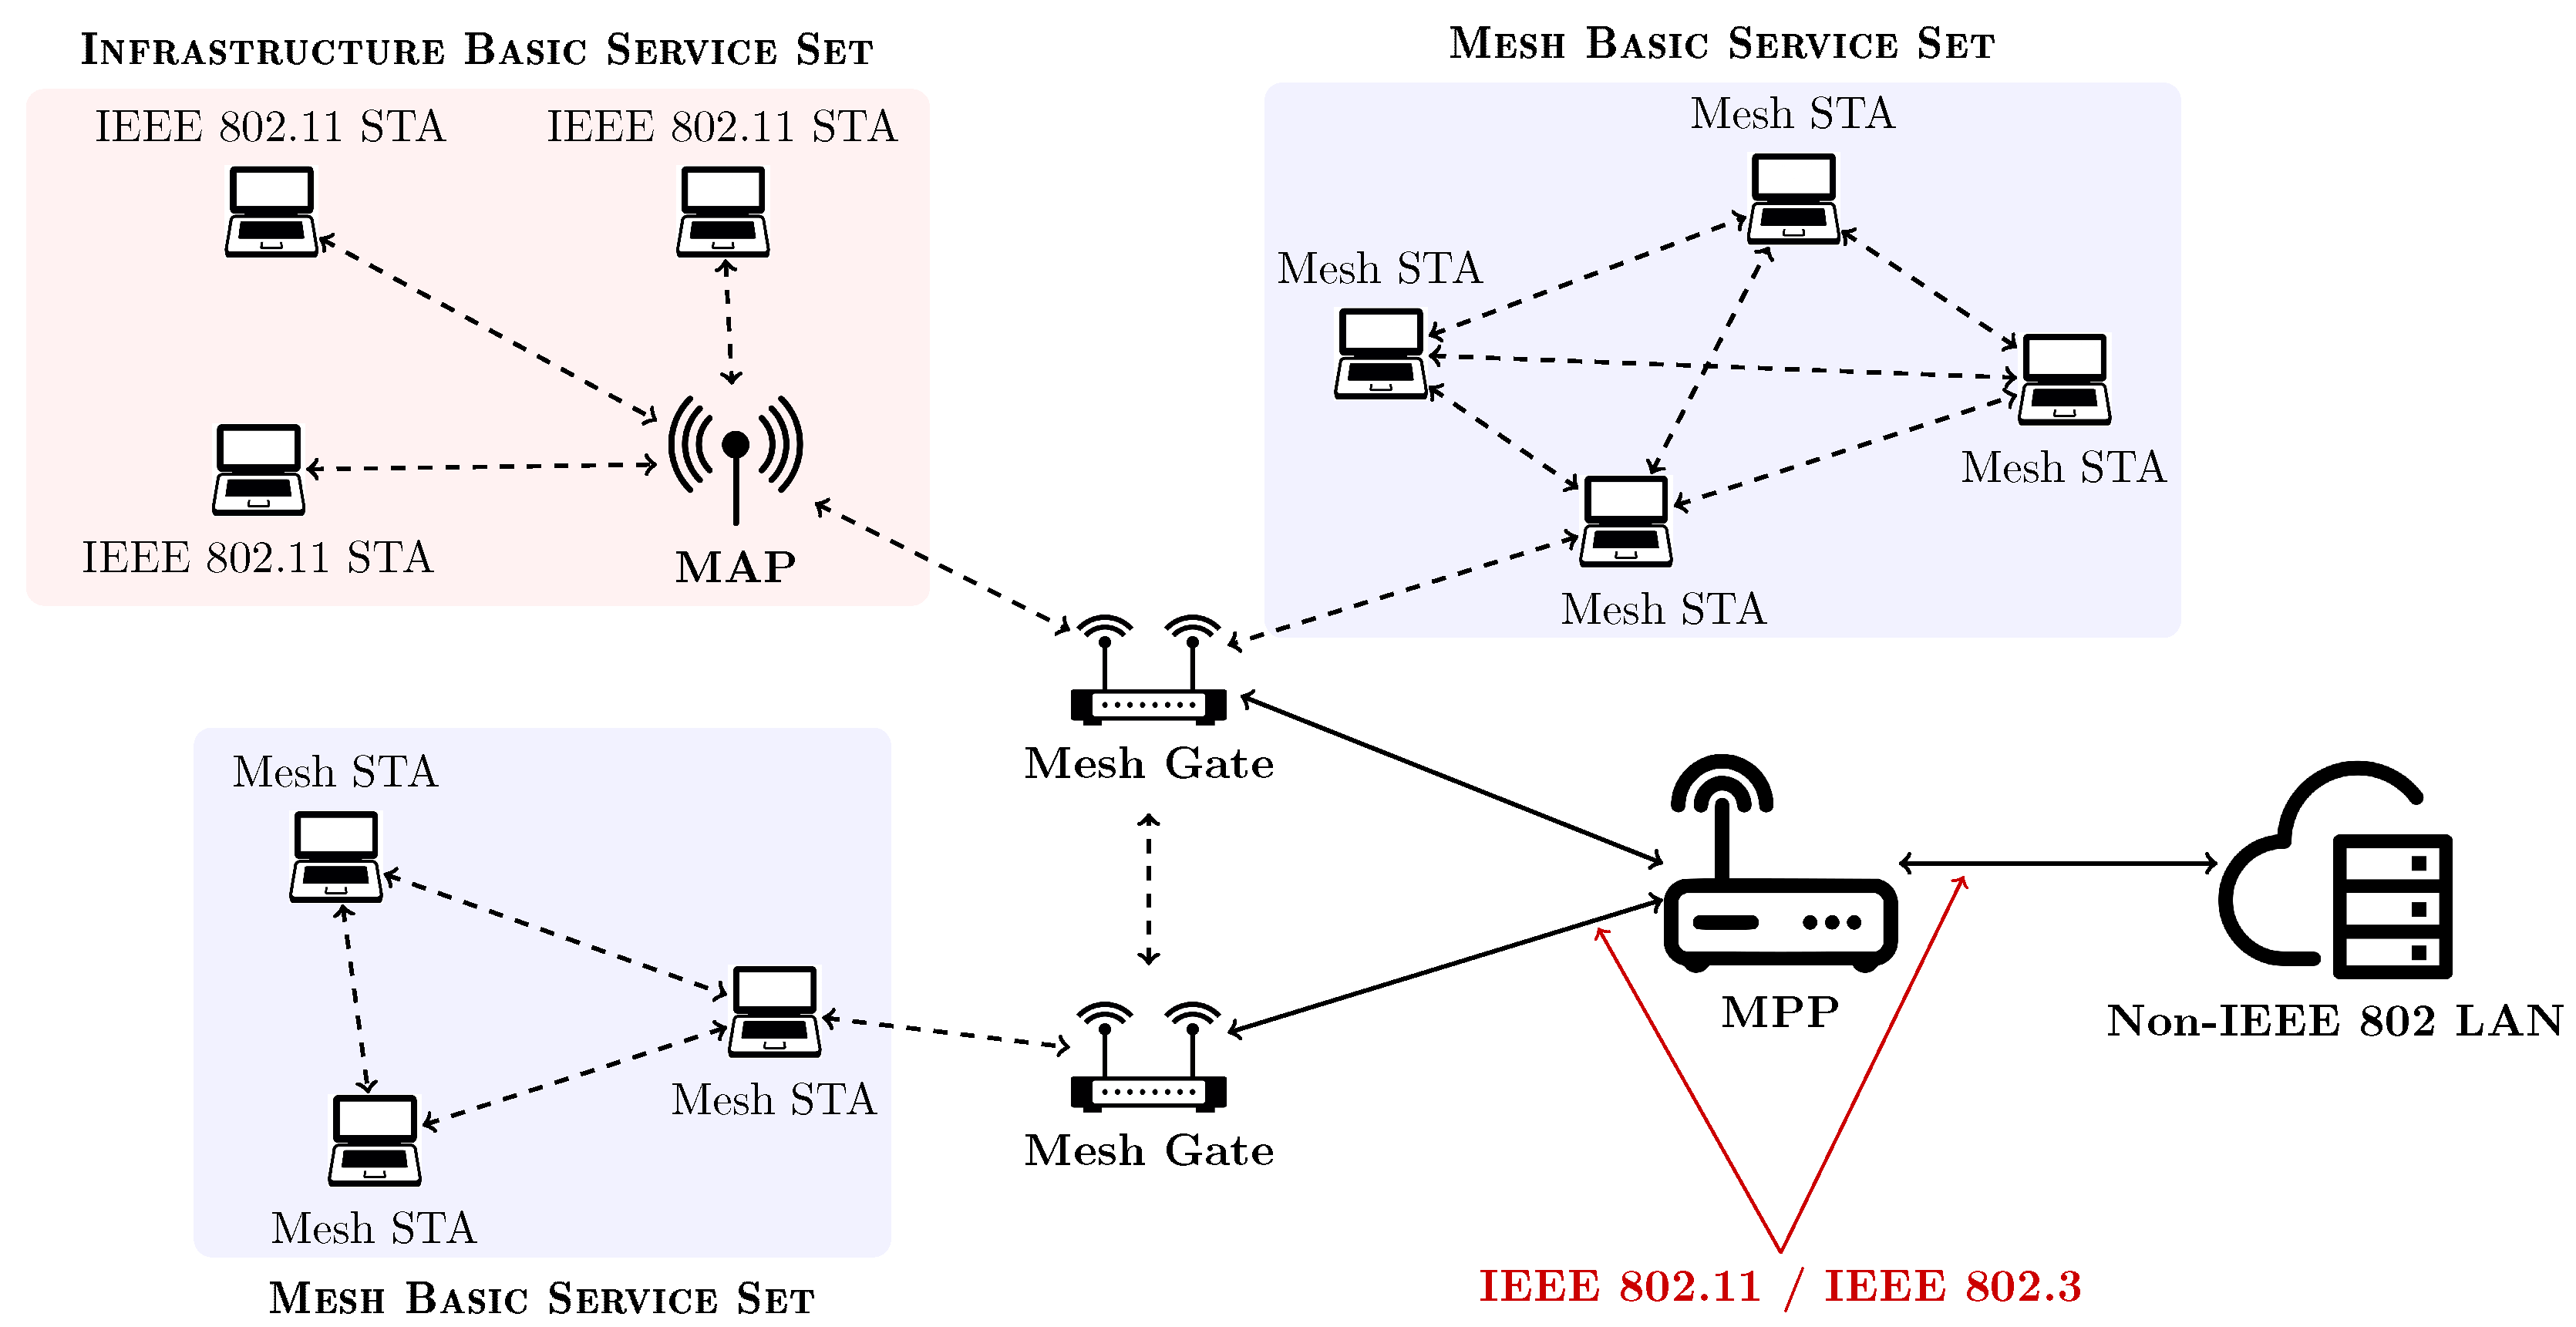
\includegraphics[width=0.9\textwidth]{MeshNetwork}
		\label{Mesh}
            \end{figure}    

            Im Falle der Integration mit anderen Netzwerktypen, wie dem \enquote*{traditionellen} IEEE 802.11 oder wenn der MBSS auf externe Netzwerke zugreifen muss, sind andere logische Komponenten erforderlich. Die Geräte, welche den Zugang zum Mesh-Netzwerk für \enquote*{traditionelle} IEEE 802.11-Stationen gewährleisten, werden als Mesh APs (MAPs) bezeichnet. Darüber hinaus werden zur Kommunikation zwischen dem Mesh Netzwerk und einem nicht-IEEE 802.11 Local Area Networks (LANs), wie beispielsweise einem kabelgebundenen LAN, weitere logische Komponenten verwendet, nämlich die Mesh Portal Points (MPPs), die die Kommunikation mit externen Entitäten ermöglichen \parencite[4\psqq]{Cilfone.2019}.  %Quelle Wireless Mesh Networking: An IoT-Oriented Perspective Survey on Relevant Technologies
            
		\section{Zigbee}
            ZigBee ist ein drahtloses Netzwerkprotokoll, das für niedrige Datenraten und niedrigen Stromverbrauch optimiert ist und hauptsächlich für die Automatisierung von Hausgeräten und anderen Geräten im IoT verwendet wird. Es wurde von der ZigBee Alliance entwickelt und basiert auf dem IEEE 802.15.4-Standard für Personal Area Networks (PANs).
            Eines der wichtigsten Merkmale von ZigBee ist seine Fähigkeit, eine große Anzahl von Geräten mit geringem Stromverbrauch zu verbinden. Es ist auch sehr skalierbar und kann Netzwerke mit Hunderten von Geräten unterstützen. Die Sicherheit ist in ZigBee gut implementiert und es bietet auch eine hohe Zuverlässigkeit und geringe Latenzzeiten.
            ZigBee wird hauptsächlich in Anwendungen verwendet, in denen niedrige Datenraten und geringer Stromverbrauch erforderlich sind, wie beispielsweise in der Steuerung von Beleuchtung, Heizung und Klimatisierung, in Sicherheitssystemen und in der Überwachung von Umweltbedingungen. Es wird auch in vielen anderen Anwendungen im Bereich des Internet der Dinge verwendet, wie beispielsweise in der Industrieautomatisierung und in Gesundheitsüberwachungssystemen \parencite[195]{Gessler.2015}. %quelle Wireless-Netzwerke für den Nahbereich: Eingebettete Funksysteme: Vergleich von standardisierten und proprietären Verfahren
	
	\chapter{Angriffsszenarien}
 %Allgemeines zum Thema Angriffsszenarien
		\section{Hacking}
            Hacking bezeichnet die Praxis in Computer- und Netzwerksysteme einzudringen, um sie ohne autorisierte Berechtigung zu nutzen oder zu verändern. Hacker haben oft das Ziel, Zugang zu sensiblen Daten zu erlangen oder das System zu beschädigen oder zu stören. Sie verwenden dazu oft spezielle Tools und Techniken, um in das System einzudringen und Sicherheitsvorkehrungen zu umgehen. Es ist wichtig, die Sicherheit von Computersystemen und -netzwerken zu verbessern und zu schützen, um sich vor Angriffen zu schützen.
			\subsection{White Hat Hacking}
                Als White Hat Hacking wird die Praxis bezeichnet, wenn es um ehere Ziele geht wie das Aufdecken von System-Schwachstellen oder wenn Sicherheitsfachleute gezielt angeheuert werden, um \enquote*{Penetrationstests} in den Netzwerke von Firmen oder Behörden durchzuführen. Dies wird auch als \enquote*{Ethical Hacking} bezeichnet \parencite[134\psq]{Sinha.2020}.
                
    
			\subsection{Black Hat Hacking}
                Im Gegensatz dazu steht das Black Hat Hacking. Hierbei handelt es sich um kriminelle Aktivitäten, mit dem Ziel Systeme zu schädigen, zu zerstören, oder Daten daraus abzuziehen. Es kann auch als Vorbereitung für andere Aktivitäten dienen, wie die Ausführung von Ransomware, wobei die Inhalte der Systeme verschlüsselt und unbrauchbar gemacht werden und nur gegen Zahlung eines Lösegelds die Daten wieder freigegeben werden \parencite[134\psq]{Sinha.2020}. 
                
                %"The Social Media Reader" Infos über Black Hat Hacking 8.Phreaks, Hackers, and Trolls

        
                
	\section{Ausnutzung von Fehlern in der Sicherheit von Routern und Smart Home Geräten}
 Kein System ist von Grund auf perfekt. Mit der Zeit werden Systeme entsprechend geupdated und Sicherheitslücken werden geschlossen. Smart Home Geräte wie Kühlschränke, Glühbirnen oder ähnliches werden jedoch häufig von sicherheitsunkundigen Personen genutzt, nach dem Kauf an Strom und Internet angeschlossen und danach nicht weiter beachtet. Dadurch bleiben Sicherheitslücken bestehen, die sich schon bei der Produktion in den Geräten befunden haben. Solche Sicherheitslücken können dann von Hackern ausgenutzt werden. In den gleichen Bereich fallen auch standardmäßig gesetzte Passwörter, die in Handbüchern stehen, bei allen Geräten gleich sind und nicht geändert werden. Die Ransomwares WannaCry und NotPetya verursachten im Jahre 2017 Milliarden an Schäden, indem sie eine Schwachstelle in der Implementierung des Server Message Block Protokols von Microsoft ausnutzten \parencite[5]{Chantzis.2021}. Zum Zeitpunkt des Angriffs war der Fehler bereits bekannt und es stand seit 2 Monaten ein Hotfix von Microsoft zur Verfügung.
 
 Im Juni 2020 veröffentliche das Fraunhofer-Institut für Kommunikation, Inforamtionsverarbeitung und Ergonomie (FKIE) einen Bericht über die Sicherheit von Home Routern. Router dienen im Privathaushalt als Verbindungspunkt der Computer und IoT-Systeme zum Internet. Es stellt gleichzeitig die erste Verteidigungslinie gegen Angriffe dar. Gleichzeitig verwaltet der Router das Kabel-Netzwerk, WLAN, Passwörter für die Verbindungen und weitere sicherheitsrelevante Einstellungen. Der Bericht listete von 127 aktuellen Routern keinen ohne Fehler. Die durchschnittliche Zeit seit dem letztem Sicherheitsupdate lag bei 378 Tagen.
\begin{figure}[H]
	\centering
	\caption{Tage seit dem letztem Sicherheitsupdate vor dem 27.03.2020}
	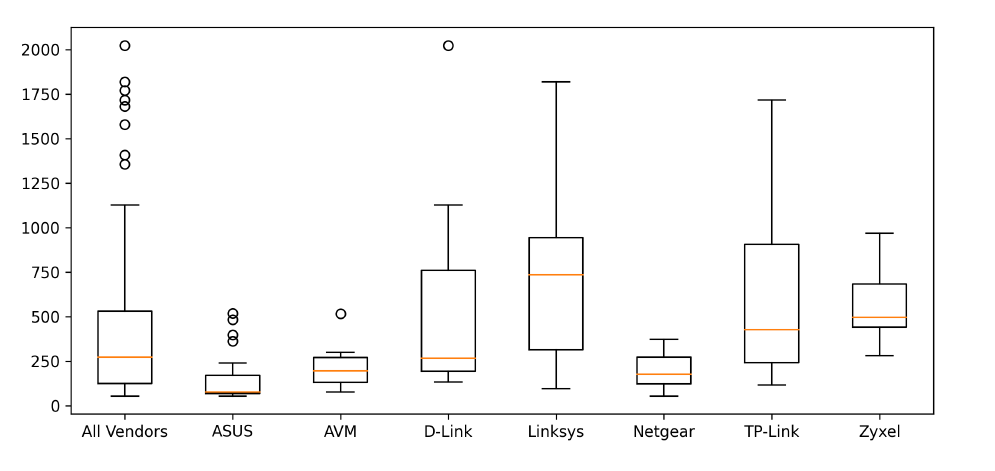
\includegraphics[width=0.9\textwidth]{Sicherheitsupdates.png}
	\label{Sicherheitsupdates}
\end{figure}
            
 Im Schnitt wurden in jeder Firmware 5 Private Keys zur Verschlüsselung und Entschlüsselung gefunden werden. Private Keys dienen in asymmetrischen Verschlüsselungsverfahren dazu Geheimtext wieder in Klartext zu übersetzen. Durch die Veröffentlichung von Private Keys werden diese wertlos und stellen ein Sicherheitsrisiko dar, da nun jeder Zugriff auf den Klartext hat. Zudem wurden in 50 Systemen fest in die Hardware integrierte Zugangsdaten gefunden, die sich größtenteils auch nicht löschen ließen. Davon waren 16 hinlänglich bekannt oder einfach zu erraten \parencite{FrauenhoferFKIE.2020}.

		\section{Spoofing}
  Beim Spoofing agieren Angreifer, als wären sie Teil des Netzwerkes oder als wären sie jemand anderes. Dies ermöglicht dem Angreifer sich zwischen zwei kommunizierende Geräte zu platzieren, die Übertragungen beider Seiten abzufangen und diese durch seine eigenen Übertragungen zu ersetzen. Diese Form wird Man-In-The-Middle-Angriff genannt.
   
\begin{figure}[H]
	\centering
	\caption{Mallory sitzt zwischen Alice und Bob und fängt die Kommunikation ab}
	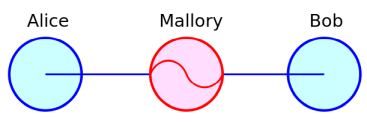
\includegraphics[width=0.6\textwidth]{MITM.png}
	\label{MITM}
    \end{figure} 
    
  Alternativ kann der Angreifer sehr viele Anfragen an einen Netzwerkteilnehmer schicken, wobei er die Daten des anfragenden Geräts fälscht. Die Antworten werden dann an diese gefälschte Adresse geschickt, mit dem Ziel diese Adresse mit den Antworten zu überlasten. Hier spricht man von einer Denial-of-Service-Attacke, oder wenn mehrere Geräte genutzt werden, um ein Ziel zu mit Antworten zu überfrachten, von einer Distributed-Denial-of-Service-Attacke.
  
		\section{Seitenkanalattacke}
  Nach Abrishami handelt es sich bei Seitenkanalattacken um nicht invasive Angriffe, da die Geräte dabei nicht zerstört oder verändert werden. Durch Beobachtung, Messungen, Abfangen von Funkdaten mit oder ohne Senden von Daten an das Gerät lassen sich Rückschlüsse auf interne Komponenten oder Berechnung durchführen. Unterschieden werden dabei sieben verschiedene Möglichkeiten der Seitenkanalattacke \parencite{Abrishamchi.2017}.
  
  Eine davon ist die Netzwerkverkehranalyse. Dabei werden die Pakete, die in einem Netzwerk von Geräten verschickt und empfangen werden, analysiert. Sender- und Empfänger\hyphen MAC\hyphen Adresse sind in jedem Paket nach IEEE 802.3 Standard im Klartext vorhanden und auslesbar. Dadurch lässt sich ermitteln welche Geräte untereinander kommunizieren. Durch die Größe der Pakete, Anzahl oder Zeitpunkte lassen sich weitere Details ermitteln.
  
  Zum Beispiel sendet ein Gerät, das auf Sprachbefehle wartet, regelmäßig Daten an einen Server, um die aufgenommenen Geräusche zu analysieren. Bei erhöhter Kommunikation des Geräts und Antworten des Servers liegt daher der Verdacht nah, dass gesprochen wird und sich mindestens eine Person im Raum befindet. Khan et. al. waren 2009 bei verschlüsselter Kommunikation in der Lage aus 10 Personen mit 70-75\% Wahrscheinlichkeit die sprechende Person zu identifizieren \parencite[70]{Khan.2010}.
		
	\chapter{Gründe für das Hacking}
 Gründe für das Angreifen von Teilen des IoT sind unterschiedlich und abhängig ob die Ziele bewusst ausgewählt werden, z.B. im Rahmen von Firmenspiongage, oder es sich um zufällige Ziele handelt, um ein Botnetzwerk aufzubauen.
 
		\section{Botnetze}
  Kleinere Gegenstände aus dem IoT haben bauartbedingt nicht die gleiche Rechenkapazität wie ein Desktop-PC oder ein Laptop/Tablet. Dies wäre auch völlig überdimensioniert. Da die Programme auf solchen Geräten gleichzeitig recht einfach sind und wenig Leistung erfordern ist jedoch freie Rechenkapazität vorhanden. Durch das Einbinden von solchen Kleinstrechnern in das Botnet kann über die reine Anzahl solcher Geräte ein profitables Botnetz entstehen. Im Bericht der BSI aus dem Jahre 2015 steht, dass im Durchschnitt pro Tag 60.000 neue Systeme pro Tag allein in Deutschland infiziert werden. Nicht alle werden in Botnetze eingebunden oder bleiben übernommen, aber es besteht Potential \parencite[30]{BundesamtfurSicherheitinderInformationstechnik.20210106}. Mit der steigenden Anzahl an IoT-Geräten seit 2015 ist auch damit zu rechnen, dass sich diese Zahl vergrößert hat. Laut Putman haben Botnetze die Möglichkeit sechsstellige Summen oder noch höhere Beträge zu erwirtschaften \parencite{Putman.2018}. 
  
		\section{Einfallstore in Netzwerke}
  Beim Angriff auf Systeme gehen Hacker meist sehr gezielt und methodisch vor. Entsprechend greifen sie nicht zuerst die am stärksten gesicherten Teile eines Netzwerkes am, um in ein System einzudringen. Sondern sie versuchen sich zuerst an den weniger gesicherten Geräten, um Zugriff zu erlangen. Sobald ein Hacker Zugang zu einem schwächer gesicherten Gerät oder einer schwächer gesicherten Komponente erhalten hat, kann er sich von dort aus weiter ausbreiten und das System schrittweise infiltrieren. Entweder indem Informationen abgegriffen werden können, die die Attacke auf eine andere Komponente erlauben. Eine andere Möglichkeit besteht darin, das schwächere Gerät oder die schwächere Komponente als Basis zu verwenden, um die eigene Identität zu verschleiern und sich als eine andere Person oder ein anderes Gerät auszugeben. Hierbei kann der Hacker andere Teile des Systems manipulieren oder steuern, ohne erkannt zu werden.
  
		\section{Ausspähen von menschlicher Anwesenheit}
  Durch die Ausnutzung von Angriffen, die auf die Anwesenheit von Personen in Gebäuden hindeuten (siehe Seitenkanalattacken) können bereits durch das Abfahren einer Straße zu vermeidende Objekte ausgemacht werden. Einbrecher wollen unbeachtet sein, und die Ermittlung im Vorfeld von Gebäuden mit anwesenden Personen vermindert entsprechend die Gefahr für diesen Personenkreis.
  
  Eine weitere Möglichkeit der Nutzung von solchen Erkenntnissen ist die Erstellung von Bewegungsprofilen von Personen. Hier sticht insbesondere die Verfolgung sogenannter Wearables (Smartwatches, Fitnesstracker o.ä.) hervor. Meist sind diese mit einem Mobiltelefon verbunden, tauschen regelmäßig Daten aus oder laden sie auf Webseiten hoch. Auf diese Weise wurde im November des Jahres 2017 eine geheime Afghanistan-Basis der US Armee enttarnt, als vom dem sozialem Fitnessnetzwerk Strava eine Heatmap mit 3 Billionen GPS-Punkten veröffentlicht wurde. Ein extrem heller Spot in einem ansonsten dunklem Gebiet in der Helmand Provinz in Afghanistan ließ dabei auf Anwesenheit schließen und die Heatmap war detailliert genug, um sogar das Layout der Basis in Erfahrung zu bringen. Kartendienste wie Google Maps zeigten an der gleichen Stelle keinerlei Aktivitäten \parencite{.20180128}. 

\begin{figure}[htpb]
	\centering
	\caption{Heatmap von Joggern in geheimer US Basis}
	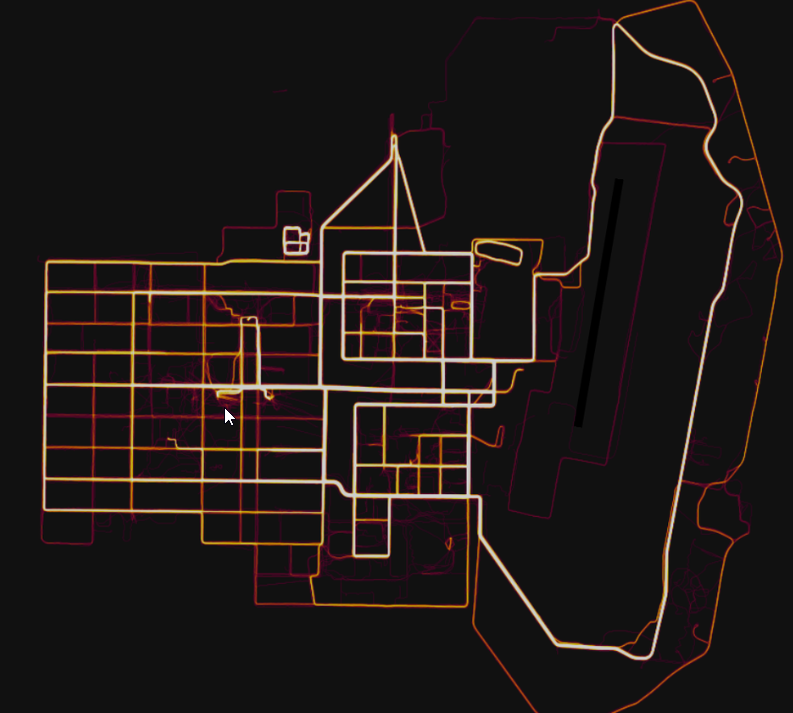
\includegraphics[width=0.9\textwidth]{Heatmap.png}
	\label{Heatmap}
\end{figure} 

        \section {Identitätsdiebstahl}
        Ein Sicherheitsrisiko, welches bei Smart Home Geräten auftreten kann, wäre das Risiko des Identitätsdiebstahls. Hierbei versuchen die Hacker Zugriff auf die persönlichen Informationen eines Benutzers zu erlangen. Eine mögliche Ursache zum Erfolg der Hacker sind die Sicherheitsprotokolle der Smart Home Geräte, welche nicht den ausreichenden Schutz bringen oder vom Benutzer des Gerätes nicht ausreichend konfiguriert worden sind. 
        Persönliche Informationen folgende Informationen sein:
        \begin{itemize}
          \item Zugangsdaten wie Benutzername, Passwörter und andere Anmeldeinformationen
          \item Finanzinformationen wie Zahlungsdaten oder Kreditkarteninformationen 
          \item Persönliche Daten wie Name, Adresse, Telefonnummer oder auch Geburtsdatum
        \end{itemize}
        
        \section{Spurenloser Einbruch in Häuser oder Wohnungen}
        Zugangssysteme mittels RFID-Tags, -Karten oder dem Mobiltelefon,  sowie biometrische Systeme haben auch in Privathaushalten Einzug erhalten und ersetzen den klassischen Schlüssel an der Haustür. Sind diese Systeme mit einer Basisstation verbunden, ist diese im Normalfall an das Internet angebunden und kann über bereits erwähnte Wege angegriffen werden, um so Zutritt zu erlangen. Es besteht aber auch die Möglichkeit mittels RFID-Lesern den Inhalt des Zugangstokens auszulesen. Dazu genügt es oft schon den Leser für 1 bis 2 Sekunden in der Nähe des RFID-Tags zu bringen. Anschließend können mittels verschiedener Programme oder eines Brute-Force-Angriffs den Inhalt der Sector Keys [Anm.: Sector Keys sind Verschlüsselungsdaten, die den Zugriff auf bestimmte Sektoren des RFID-Chips erlauben] ausgelesen werden und so eine funktionierende Kopie des Zugangstokens repliziert werden. Mit diesem kann dann die Haustür normal geöffnet werden, ohne das Einbruchsspuren zurück bleiben. Eventuell vorhandene Alarmsysteme können zudem häufig mit einem Störsender überlagert werden, indem ein weißes Rauschen auf den verwendeten Frequenzen gesendet wird.

        Ein entsprechender Angriff inklusive verwendeter Soft- und Hardware wird in \citetitle{Chantzis.2021} auf den Seiten 372-379 ausführlich dargelegt.

    \chapter{Schutzmaßnahmen}
    Da immer mehr Menschen sich Smart Home Geräte anschaffen und benutzen steigt das auch das Potenzial von einer Hackerattacke betroffen zu sein. Immer mehr Geräte sind miteinander und dem Internet verbunden und übertragen sensible persönliche Informationen von einem selbst. Aus diesem Grund ist es Ratsam sich mit verschiedenen Schutzmaßnahmen auseinander zu setzen um das Risiko von einer Hackerattacke betroffen zu sein zu minimieren. Dabei hilft es sehr Smart Home Geräte von vertrauenswürdigen Herstellen zu kaufen, denn dort ist das Risiko am geringsten das Fremd-Hard- oder Software mit verbaut ist und man kann sich sicher sein, dass das Gerät regelmäßig mit Sicherheitspatches versorgt wird. Bei Kauf sollte dabei drauf geachtet werden, dass das Gerät, beziehungsweise der Hersteller, sicherheitszertifiziert ist. Es sollte zusätzlich überprüft werden, ob für ein Smart Home Gerät Updates verfügbar sind. Mit den Updates können Sicherheitslücken geschlossen und die Sicherheit des Smart Home Systems verbessert werden. Eine weitere Schutzmaßnahme wäre die Verwendung von starken Passwörtern. Es sollte dabei vermieden werden dasselbe Passwort für mehrere Geräte zu verwenden. Dabei gilt es auch, dass ein Smart Home Gerät nur so sicher wie sein Netzwerk ist. Hier sollte ebenfalls sichergestellt werden, dass das WiFi-Netzwerk ein sicheres Passwort verwendet. Um das Risiko weiter zu minimieren besteht die Möglichkeit seine Smart Home Geräte zu überwachen. Mit speziellen Tools ist es möglich den Netzwerkverkehr zu überwachen und sollte einem dabei etwas Verdächtiges auffallen, empfiehlt es sich das Gerät vom Netzwerk zu trennen.

   Allgemein gilt es sich im Internet mit Vorsicht zu bewegen. Wenn ein Link oder eine Website nicht vertrauenswürdig aussieht, dann empfiehlt es sich nicht drauf zu klicken. Oftmals gelangt so Schadsoftware auf ein Gerät und somit ins Netzwerk. 
        
	\chapter{Fazit}
 Smart Home Geräte befinden sich auf dem Vormarsch und immer mehr Haushalte in Deutschland werden damit ausgestattet. Gleichzeitig steigt aber nicht die Sicherheit der Geräte, sondern sie sind weithin anfällig für Angriffe, weil \textquote[{\cite[6]{Chantzis.2021}}]{the economics of IoT manufacturing drive device costs [...] to a minimum, often making security an expensive afterthought}. Das Hacking von Smart Home Geräten stellt daher eine wachsende Bedrohung dar, da immer mehr Geräte miteinander und mit dem Internet verbunden sind. Hacker können Schwachstellen in diesen Geräten ausnutzen, um persönliche Informationen zu stehlen, die Privatsphäre des Benutzers zu verletzen oder sogar Kontrolle über das Gerät zu erlangen.
 
 Um das Risiko des Hackings von Smart Home Geräten zu minimieren, sollten Benutzer sicherheitsbewusste Methoden wie die Verwendung starker Passwörter und die Aktualisierung von Firmware und Sicherheitspatches anwenden. Es ist auch wichtig, Geräte von vertrauenswürdigen Herstellern zu kaufen und darauf zu achten, dass sie die neuesten Sicherheitsstandards erfüllen.
 Hersteller von Smart Home Geräten sollten auch sicherstellen, dass ihre Geräte sicher und robust sind, indem sie regelmäßig Sicherheitsupdates durchführen und schnell auf bekannte Schwachstellen reagieren. Es ist auch wichtig, klare Datenschutzrichtlinien zu haben und Benutzer über alle Daten zu informieren, die von ihren Geräten erfasst werden.

 Black Hat Hacker sind eher daran interessiert ungeschützte Smart Home Geräte zu übernehmen und in ihre Botnetzwerke einzubinden. Jedoch sind auch direkt Angriffe auf Wohnung denk- und durchführbar. Im Bereich der medizinischen Produkte, die zwar eher in den Bereich der Wearables gehören, anstatt der Smart Home Geräte, ist die Gefahr umso größer und die Sicherheit sollte hier eine der höchsten Prioritäten einnehmen, um Menschen vor körperlichem Schaden zu bewahren.

 Denkbar sind drei verschiedene Szenarien, wie es in Zukunft mit diesem Thema weitergehen kann. Die Benutzer arrangieren sich mit dem Status quo. Übernahmen von Smart Home Geräten werden zum Alltag, ohne das weiter darüber nachgedacht wird. Als zweite Möglichkeit besteht, dass die Nutzer selbst zusätzliche Sicherheitsmaßnahmen ergreifen und die Produkte an den eigenen Bedarf angepasst sichern. Oder als dritte Option, dass die Hersteller bessere Sicherheitsoptionen in die Gegenstände integrieren, beziehungsweise die Sicherheit besser implementieren \parencite[6]{Chantzis.2021}.

\newpage %Abschluss Inhalt - Neue Seite für Anhänge
%\nocite{*}
\printbibliography* %Erzeuge Literaturverzeichnis
\appendix %Anhänge
\end{document}
